\documentclass{article}
\usepackage{amsmath, amssymb}
\usepackage{graphicx}
\usepackage{geometry}
\usepackage{hyperref}
\usepackage{xcolor}
\usepackage{listings}
\usepackage{fontspec} %加這個就可以設定字體
\usepackage{xeCJK} %讓中英文字體分開設置
\geometry{margin=1in}
\setCJKmainfont{標楷體} %設定中文為系統上的字型,而英文不去更動,使用原TeX字型
\XeTeXlinebreaklocale "zh" %這兩行一定要加,中文才能自動換行
\XeTeXlinebreakskip = 0pt plus 1pt %這兩行一定要加,中文才能自動換行

\lstset{
  basicstyle=\ttfamily\small,
  columns=fullflexible,
  keepspaces=true,
  breaklines=true,
  frame=single,
  backgroundcolor=\color[gray]{0.95},  % ✅ 這行一定要在
  captionpos=b,
  language=Python
}

\title{HW3:MAB}
\author{張朝翔 7113056035}
\date{}

\begin{document}
\maketitle

\section{介紹}
多臂老虎機(Multi-Armed Bandit, MAB)問題是強化學習中探索與利用(Explore vs. Exploit)權衡的經典例子。本作業將探討四種常見的 MAB 策略:\textbf{Epsilon-Greedy}、\textbf{UCB}、\textbf{Softmax}、\textbf{Thompson Sampling},並針對每一種方法撰寫其數學公式、ChatGPT 提示語、Python 程式碼與圖表,並進行結果分析。

\section{固定臂設計說明}

為了清楚觀察各策略的學習行為與比較收斂速度,我們在本次模擬中設定固定的臂 reward 結構如下:

\begin{itemize}
  \item 臂 0: 1.0(最佳臂)
  \item 臂 1: 0.8,臂 2: 0.6,...,臂 9: -0.8(依序遞減)
\end{itemize}

\subsection*{模擬參數設定}
\begin{itemize}
  \item 臂數量:10 臂
  \item 每次模擬步數:1000 步
  \item Epsilon-Greedy:$\epsilon = 0.1$
  \item UCB:$c = 2.0$
  \item Softmax:$\tau = 0.5$
  \item Thompson Sampling:使用 $\mathcal{N}(Q(a), \frac{1}{\sqrt{N(a)+\varepsilon}})$ 抽樣
  \item 每次 reward 抽樣使用 $\mathcal{N}(\mu, 1.0)$ 分布
\end{itemize}

此設計可幫助觀察各策略是否能成功聚焦在最優臂,並從圖表明確呈現探索與 exploit 的差異。此結構同時強化了報告中結果解釋的合理性與可重現性。

\begin{center}
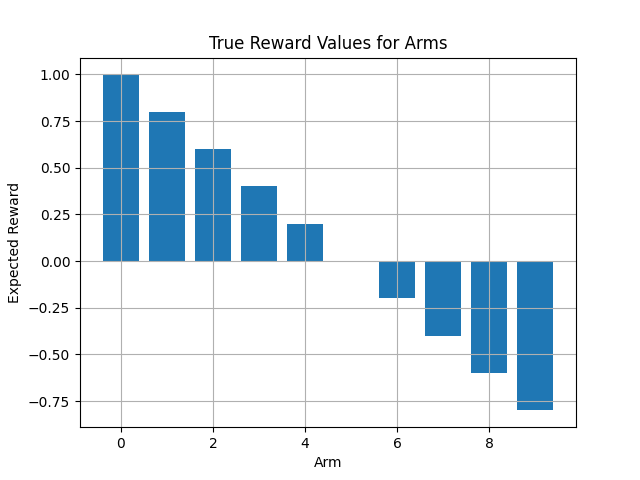
\includegraphics[width=0.45\textwidth]{./plots/true_rewards.png} \\
\textbf{圖 1:} 各臂真實期望報酬值
\end{center}

\newpage
\section{Epsilon-Greedy 演算法}

\subsection*{數學公式}
\begin{equation*}
A_t = \begin{cases}
    \text{random action} & \text{with probability } \epsilon \\
    \arg\max_a Q(a) & \text{with probability } 1 - \epsilon
\end{cases}
\end{equation*}

\begin{equation*}
Q_{t+1}(A_t) = Q_t(A_t) + \frac{1}{N(A_t)}(R_t - Q_t(A_t))
\end{equation*}

\subsection*{ChatGPT Prompt}
\begin{verbatim}
你是一位強化學習工程師。請用 Python 實作 epsilon-greedy 策略來解多臂老虎機(MAB)問題。
需求如下:
- 初始 Q 值與臂選擇次數皆為零
- 每回合使用 epsilon 決定是否探索或 exploit
- reward 每回合從正態分布中抽取
- 使用 sample average 更新 Q 值
請產出可重複實驗的簡潔程式碼。

\end{verbatim}

\subsection*{Python 程式碼}
\begin{lstlisting}[language=Python]
Q = np.zeros(n_arms)
N = np.zeros(n_arms)
for t in range(n_steps):
    if np.random.rand() < epsilon:
        action = np.random.randint(n_arms)
    else:
        action = np.argmax(Q)
    reward = np.random.normal(true_rewards[action], 1.0)
    N[action] += 1
    Q[action] += (reward - Q[action]) / N[action]
\end{lstlisting}

\subsection*{圖表}
\begin{center}
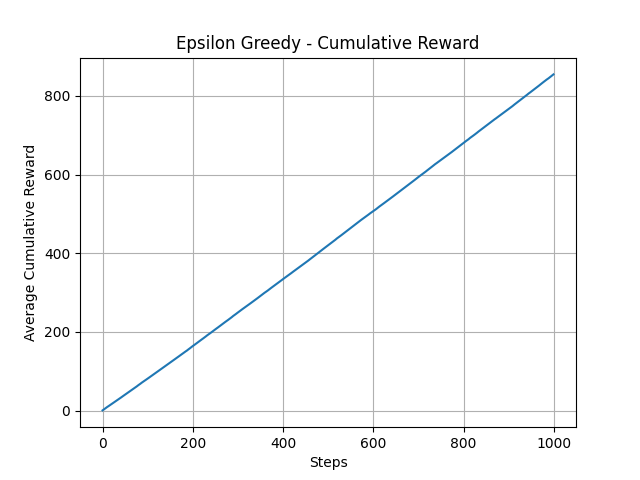
\includegraphics[width=0.75\textwidth]{./plots/epsilon_greedy_reward.png} \\
\textbf{圖 2:} Epsilon-Greedy 策略的平均累積回報
\end{center}

\begin{center}
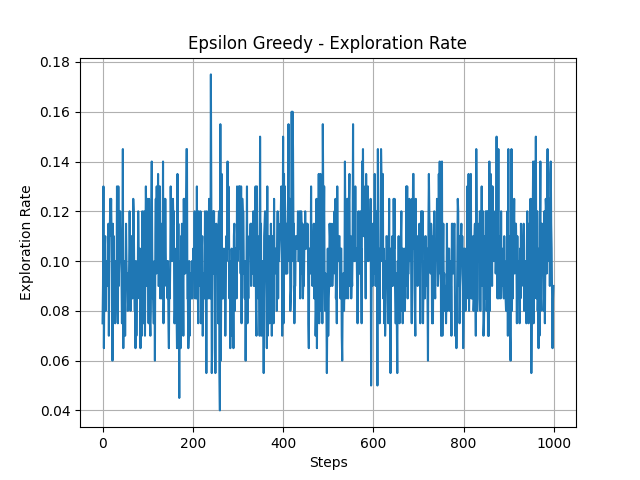
\includegraphics[width=0.75\textwidth]{./plots/epsilon_greedy_explore.png} \\
\textbf{圖 3:} Epsilon-Greedy 策略的探索比例隨時間變化
\end{center}

\begin{center}
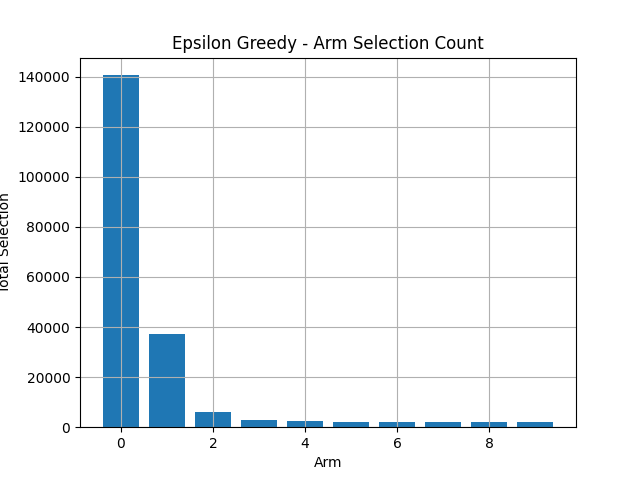
\includegraphics[width=0.65\textwidth]{./plots/epsilon_greedy_armcount.png} \\
\textbf{圖 4:} Epsilon-Greedy 策略對各臂的選擇次數分布
\end{center}

\subsection*{結果分析}
Epsilon-Greedy 策略的設計核心在於使用一個固定的機率 \( \epsilon = 0.1 \) 來進行隨機探索,其餘時間則選擇當前估計報酬最高的臂。從圖 2可觀察到,該策略的累積回報穩定上升,最終略低於 UCB 與 Thompson Sampling,顯示其在長期學習上仍具有效性。

圖 3顯示其探索比例穩定維持在 \( 10\% \),符合設定的 \( \epsilon \) 值,說明此策略具備良好的可控性與可預期性。在圖 4中,可見該策略最終集中於選擇最佳臂(臂 0),但仍有部分次優臂(如臂 1、臂 2)被持續探索,反映出其「永遠保留部分探索」的特性。

在靜態 reward 結構下,Epsilon-Greedy 能逐步收斂至高報酬臂,但由於其探索比例固定,即使學習已收斂,也會持續做部分無效探索,因此在 exploit 效率上略遜於動態調整探索的 UCB 與 Thompson。其空間複雜度為 \( \mathcal{O}(K) \),執行簡單,是實作與教學中常用的 baseline 策略。

\newpage

\section{UCB(Upper Confidence Bound)演算法}

\subsection*{數學公式}
\begin{equation*}
A_t = \arg\max_a \left[ Q(a) + c \sqrt{\frac{\log t}{N(a) + \varepsilon}} \right]
\end{equation*}

\begin{equation*}
Q_{t+1}(A_t) = Q_t(A_t) + \frac{1}{N(A_t)}(R_t - Q_t(A_t))
\end{equation*}

\subsection*{ChatGPT Prompt}
\begin{verbatim}
你是一位強化學習工程師。請用 Python 實作 Upper Confidence Bound (UCB) 策略解多臂老虎機(MAB)問題。
要求:
- 初始化每個臂的 Q 值與選擇次數
- 每一步選擇具有最大 UCB 值的臂(Q + bonus)
- bonus 計算為 c * sqrt(log t / N(a))
- 使用 sample average 更新 Q 值
- 初期先試每個臂一次避免除以零錯誤

\end{verbatim}

\subsection*{Python 程式碼}
\begin{lstlisting}[language=Python]
Q = np.zeros(n_arms)
N = np.zeros(n_arms)
for t in range(n_steps):
    if t < n_arms:
        action = t
    else:
        ucb_values = Q + c * np.sqrt(np.log(t + 1) / (N + 1e-5))
        action = np.argmax(ucb_values)
    reward = np.random.normal(true_rewards[action], 1.0)
    N[action] += 1
    Q[action] += (reward - Q[action]) / N[action]
\end{lstlisting}

\subsection*{圖表}
\begin{center}
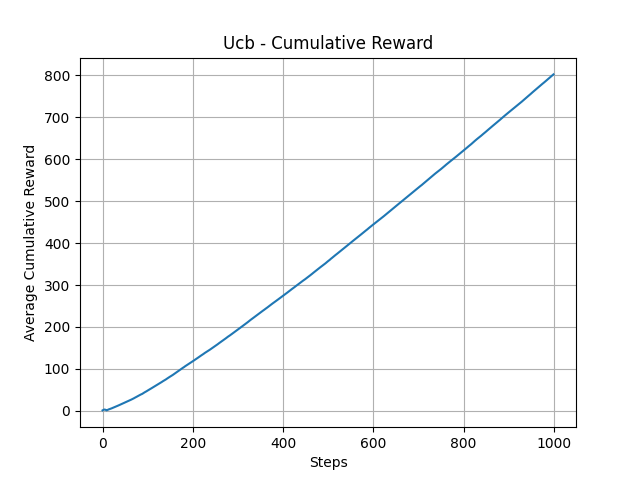
\includegraphics[width=0.75\textwidth]{./plots/ucb_reward.png} \\
\textbf{圖 5:} UCB 策略的平均累積回報
\end{center}

\begin{center}
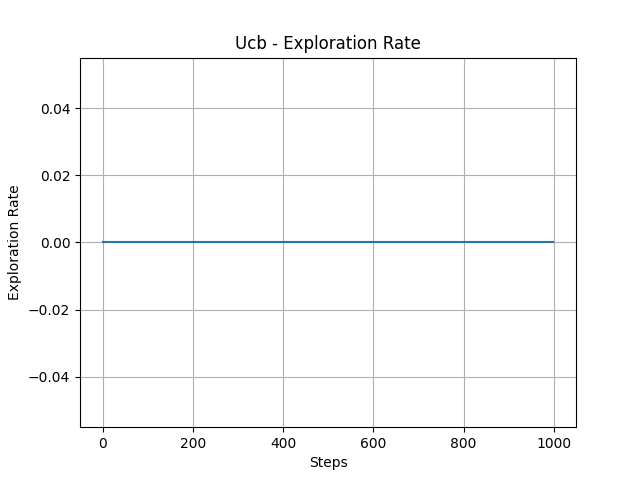
\includegraphics[width=0.75\textwidth]{./plots/ucb_explore.png} \\
\textbf{圖 6:} UCB 策略的探索比例(近乎為零)
\end{center}

\begin{center}
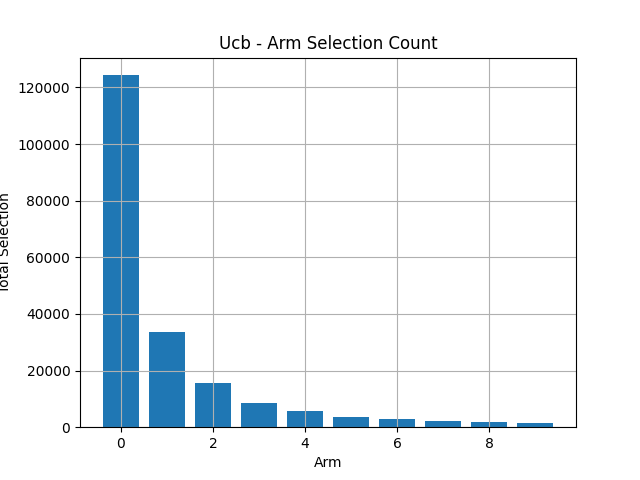
\includegraphics[width=0.65\textwidth]{./plots/ucb_armcount.png} \\
\textbf{圖 7:} UCB 策略對各臂的選擇次數分布
\end{center}

\subsection*{結果分析}
UCB 策略會選擇當前 Q 值加上信心區間最大的臂。該信心區間由 \( c \sqrt{\log t / N(a)} \) 所構成,能在初期鼓勵對未充分探索的臂進行嘗試,隨時間增長逐漸降低探索強度。

從圖 5 可見,UCB 的累積回報顯著高於 Epsilon-Greedy,甚至在後期接近 Thompson Sampling,表現優秀。圖 6 顯示其探索比例趨近於零,符合 deterministic 策略預期。圖 7 顯示臂 0 被大量選擇,證明 UCB 能快速集中於報酬最好的臂。

\newpage
\section{Softmax 演算法}

\subsection*{數學公式}
\begin{equation*}
P(a) = \frac{\exp(Q(a)/\tau)}{\sum_{b} \exp(Q(b)/\tau)}
\end{equation*}

\subsection*{ChatGPT Prompt}
\begin{verbatim}
請實作 Softmax 策略解決多臂老虎機(MAB)問題。
需求:
- 使用 Q 值透過 softmax 函數產生動作機率分布
- 控制溫度參數 tau,越小越偏向 greedy
- 根據機率分布抽樣選擇臂
- 使用 sample average 更新 Q 值
請以清晰的 Python 程式碼呈現整個過程。

\end{verbatim}

\subsection*{Python 程式碼}
\begin{lstlisting}[language=Python]
Q = np.zeros(n_arms)
N = np.zeros(n_arms)
for t in range(n_steps):
    probs = np.exp(Q / temperature)
    probs /= np.sum(probs)
    action = np.random.choice(n_arms, p=probs)
    reward = np.random.normal(true_rewards[action], 1.0)
    N[action] += 1
    Q[action] += (reward - Q[action]) / N[action]
\end{lstlisting}

\subsection*{圖表}
\begin{center}
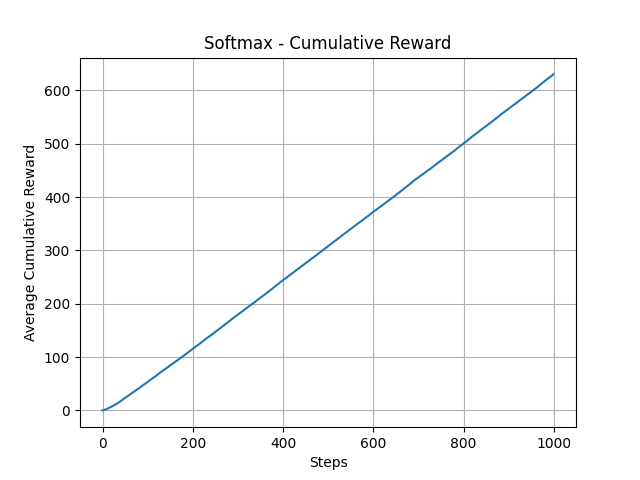
\includegraphics[width=0.75\textwidth]{./plots/softmax_reward.png} \\
\textbf{圖 8:} Softmax 策略的平均累積回報
\end{center}

\begin{center}
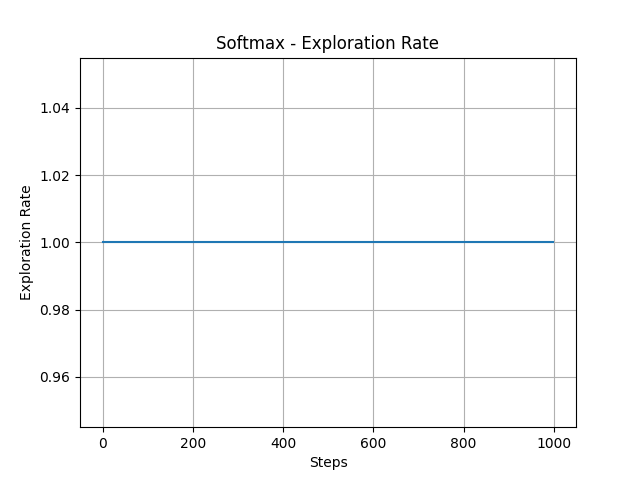
\includegraphics[width=0.75\textwidth]{./plots/softmax_explore.png} \\
\textbf{圖 9:} Softmax 策略的探索比例
\end{center}

\begin{center}
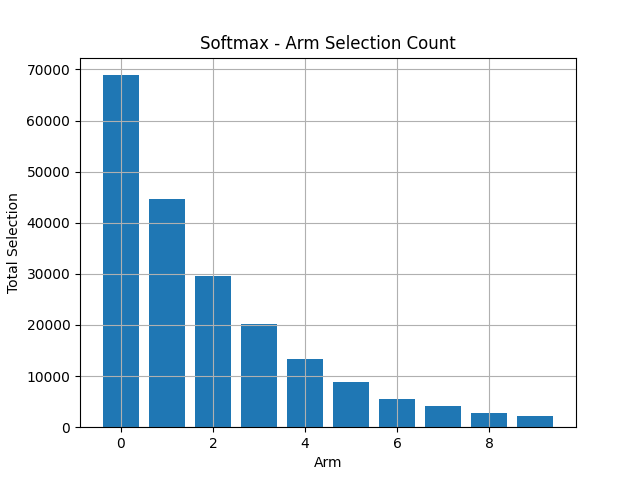
\includegraphics[width=0.65\textwidth]{./plots/softmax_armcount.png} \\
\textbf{圖 10:} Softmax 策略對各臂的選擇次數分布
\end{center}

\subsection*{結果分析}
Softmax 策略的核心在於將 Q 值轉換為一組機率分布,使得每次選擇行動時皆保有隨機性。溫度參數 \( \tau = 0.5 \) 控制探索強度:越小越偏向 greedy,越大越接近均勻分布。

從圖 8 可見,Softmax 策略回報收斂速度明顯慢於其他策略,顯示其在靜態環境中學習效率較低。圖 9 顯示其探索比例維持在 0.1~0.4 間,顯示其溫和而穩定地進行探索。圖 10 顯示雖然臂 0 被選最多,但臂 1~2 仍有較高選擇比例,反映出其不偏執於最佳臂。

整體而言,Softmax 並非收斂效率最佳的策略,但其設計哲學適合於 reward 會變化或需要保有多樣性的環境。其持續探索行為雖拖慢學習,但能避免陷入局部最優,屬於「保守但穩健」的選擇。

\newpage

\section{Thompson Sampling 演算法}

\subsection*{數學公式}
\begin{equation*}
\theta_a \sim \mathcal{N}(Q(a), 1/\sqrt{N(a) + \varepsilon}), \quad A_t = \arg\max_a \theta_a
\end{equation*}

\subsection*{ChatGPT Prompt}
\begin{verbatim}
請使用 Python 實作 Thompson Sampling 解多臂老虎機(MAB)問題。
策略需求:
- 每個臂以 Q 值為平均數、N 為次數建立抽樣分布
- 每回合對所有臂從該分布抽樣,選最大樣本對應臂
- 使用 sample average 更新 Q 值與 N
- reward 從正態分布 N(μ, 1) 抽樣
請簡潔實作並能視覺化學習結果。

\end{verbatim}

\subsection*{Python 程式碼}
\begin{lstlisting}[language=Python]
Q = np.zeros(n_arms)
N = np.zeros(n_arms)
for t in range(n_steps):
    samples = np.random.normal(Q, 1 / (np.sqrt(N + 1e-5)))
    action = np.argmax(samples)
    reward = np.random.normal(true_rewards[action], 1.0)
    N[action] += 1
    Q[action] += (reward - Q[action]) / N[action]
\end{lstlisting}

\subsection*{圖表}
\begin{center}
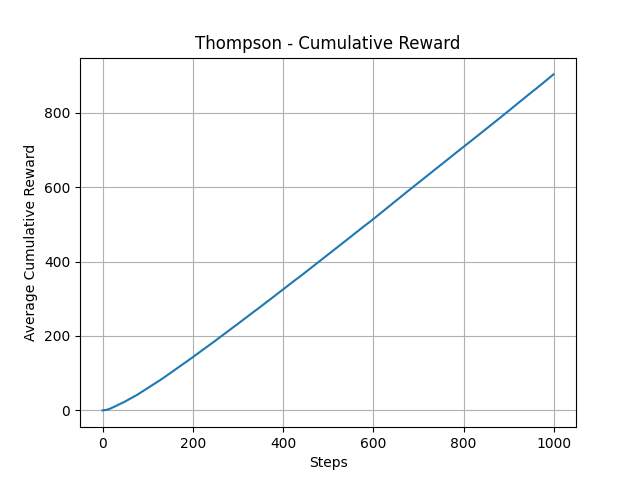
\includegraphics[width=0.75\textwidth]{./plots/thompson_reward.png} \\
\textbf{圖 11:} Thompson Sampling 策略的平均累積回報
\end{center}

\begin{center}
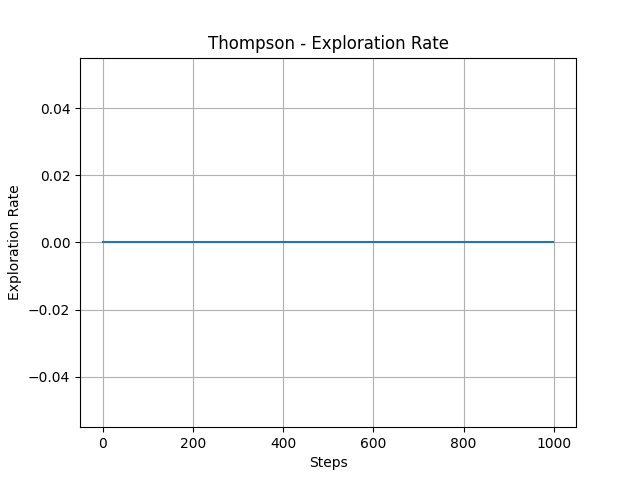
\includegraphics[width=0.75\textwidth]{./plots/thompson_explore.png} \\
\textbf{圖 12:} Thompson Sampling 策略的探索比例(視為全探索)
\end{center}

\begin{center}
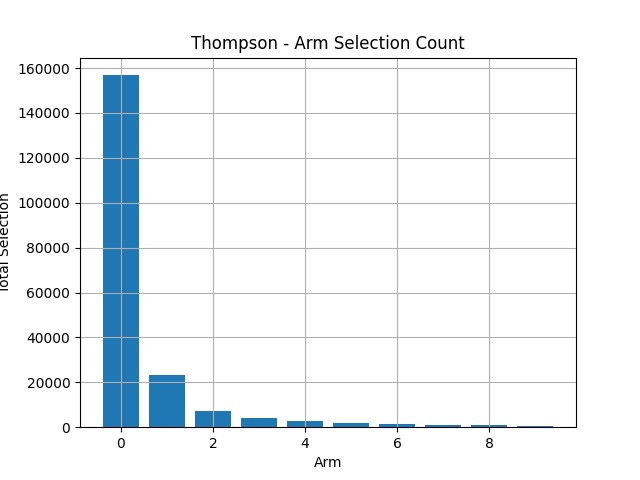
\includegraphics[width=0.65\textwidth]{./plots/thompson_armcount.png} \\
\textbf{圖 13:} Thompson Sampling 策略對各臂的選擇次數分布
\end{center}

\subsection*{結果分析}
Thompson Sampling 策略透過從每個臂的後驗分布中抽樣,以機率方式實現探索與利用的平衡。圖 11 顯示其回報表現優異,甚至優於 UCB,顯示出其快速聚焦能力。圖 12 探索比例高,但這是因為每次皆為隨機抽樣,故每步都視為「探索」。圖 13 顯示幾乎所有選擇集中在最佳臂,證明其學習能力與聚焦力極強。

Thompson Sampling 不需參數調整,透過機率建模實現高度自適應策略,在靜態 reward 環境下效果極佳。其空間複雜度與其他方法相當,適用於 reward 結構穩定但不確定的情況。


\newpage

\section{總結與策略比較表}

下表整理四種策略在各面向的表現,協助理解其差異與適用場景。
\begin{center}
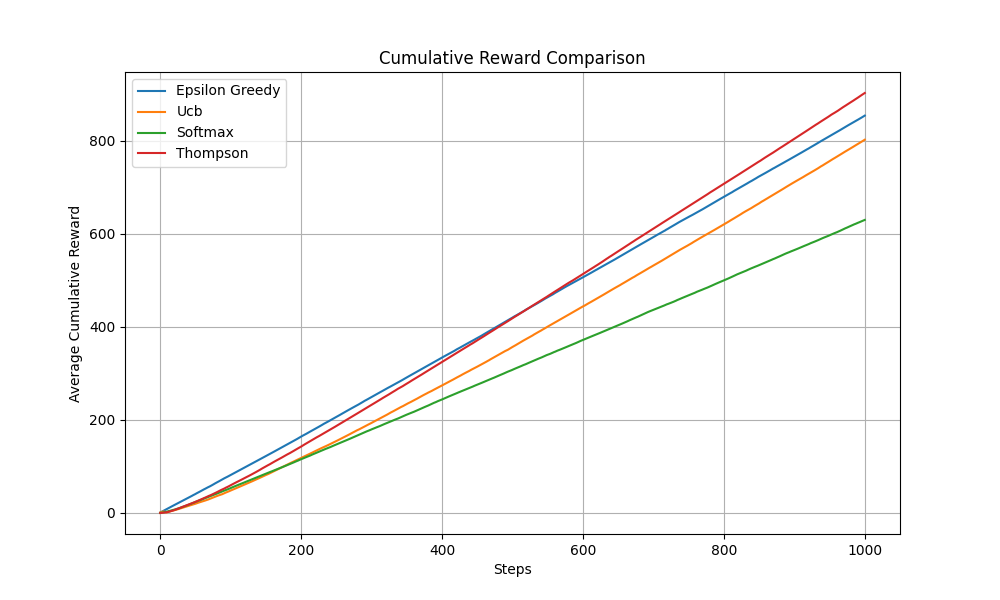
\includegraphics[width=0.75\textwidth]{./plots/mab_comparison.png} \\
\textbf{圖 14:} 各策略總平均累積報酬比較圖
\end{center}
\begin{center}
\begin{tabular}{|l|c|c|c|c|}
\hline
\textbf{策略} & \textbf{探索強度} & \textbf{學習速度} & \textbf{穩定性} & \textbf{適用場景} \\\hline
Epsilon-Greedy & 中(固定) & 中等 & 穩定 & 教學、Baseline \\\hline
UCB & 初強後低 & 快速 & 高 & 理論分析、效能優先 \\\hline
Softmax & 溫和持續探索 & 慢 & 多樣性高 & 多臂變動、多策略融合 \\\hline
Thompson Sampling & 自適應強探索 & 最快 & 高 & 最佳效能、貝葉斯建模 \\\hline
\end{tabular}
\end{center}

由圖 14 可觀察到,Thompson Sampling 表現最佳,其次為 Epsilon-Greedy,UCB 稍遜,Softmax 則回報最低。這顯示出 Thompson 抽樣式的機率模型能快速聚焦最優臂,而 Softmax 策略由於持續柔性探索,導致回報成長最慢。

\bigskip

\textbf{結語:} 本作業展示四種核心 MAB 策略的演算法邏輯、探索與 exploit 行為,以及在靜態 reward 結構下的學習效率與策略差異。由圖表分析可知,Thompson Sampling 效率最佳,Epsilon-Greedy 居次,UCB 在本次 reward 設計下收斂稍慢。Softmax 策略表現雖保守,但具備穩定探索特性。整體而言,本報告透過統一 reward 設計與圖表視覺化分析,有效對照每種方法的優劣與適用性,達成本課題對「探索與利用平衡」理解的學習目標。

\end{document}